\subsection{Failure Modes and Fallback}
\label{sec:fallback}

A control point on the hot path has to say what happens when it is
slow, down, or unable to decide. \system's answers are explicit and
configured, not emergent.
Figure~\ref{fig:fallback} summarises the four cases below.

\begin{figure*}[t]
    \centering
    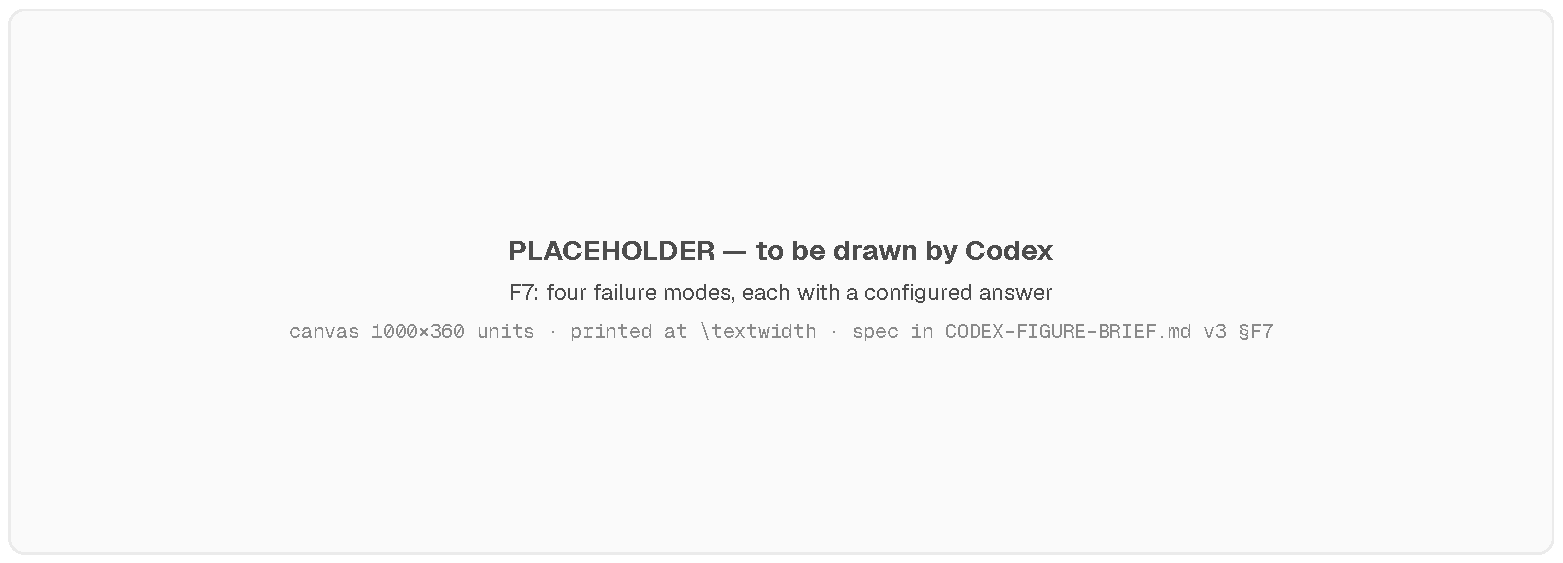
\includegraphics[width=\textwidth]{images/fallback.pdf}
    \caption{Four failure modes and the configured answer to each: what the agent sees, and what the operator sees. Every branch is a switch an operator sets; the decision pipeline (L1, L2, L$_\mathrm{p}$, policy) needs no model in any of them.}
    \label{fig:fallback}
\end{figure*}

\paragraph{When the gateway is unreachable.}
The SDK's blocking check carries a 3\,s timeout. What happens on timeout
is a single switch, \texttt{fail\_open}: open means the call proceeds, and its trace carries no gateway verdict; closed means it is refused with
\texttt{gateway-unreachable} as the reason. The shipped default is open,
because an SDK that silently stops an agent when a sidecar restarts is
the first thing an operator removes; the compatibility runs in
Appendix~\ref{app:compat} set it closed, which is what we recommend once a
deployment is past evaluation. Traces are never lost to an outage: the
transport retries with exponential backoff (0.5\,s base, 30\,s cap), a
circuit breaker opens after five consecutive failures so that sends fail
fast instead of stalling the agent, and while it is open traces go to a
local disk queue that is replayed on the next start. The in-memory queue is bounded (10{,}000 traces); past it, traces spill to the same disk queue (or are dropped, if the local fallback is off), so a long outage costs disk, not memory.

\paragraph{When a person does not answer.}
A held call expires at the gateway after ten minutes as a block, and the agent receives that block in the same slot an approval would have arrived in; with the SDKs' defaults the agent stops waiting at five minutes and reports a block itself. On the
egress-proxy path, which cannot hold an inline HTTP response, a
\texttt{pending} decision is applied as a block and the audit record is
tagged so the operator sees why.

\paragraph{When a compensator fails.}
Recovery (\S\ref{sec:recovery}) depends on compensating actions that are
themselves calls to the operator's systems. A compensator that fails
despite retries lands in a dead-letter queue the operator can inspect, retry or discard through the gateway's API (\texttt{/api/v1/rollback/dlq}; the Cockpit has no view of it yet), so a failed undo is a recorded item, not a silent inconsistency.

\paragraph{When there is no model.}
Three features call a language model: the natural-language policy compiler, the alignment auditor and the trace judge (\S\ref{sec:judge}). The compiler and the auditor select a client by a fixed priority---a local OpenAI-compatible endpoint (vLLM, Ollama, LocalAI) if one is configured, then Anthropic, then OpenAI---and a single switch, \texttt{AEGIS\_OFFLINE}, severs their cloud calls without touching the keys. Two paths do not yet honour it: the trace judge, which takes its provider and key per request, and the Cockpit's own natural-language policy page, which calls a cloud API directly; an air-gapped deployment leaves both unconfigured. With no model at all the
policy compiler falls back to a heuristic backend, and the decision
pipeline itself never needed one: L1, L2, L$_\mathrm{p}$ and the policy
DSL run without a model call.
